\documentclass[journal]{IEEEtran}
\usepackage[pdftex]{graphicx}
\usepackage[table]{xcolor}
\usepackage{parskip}
\usepackage{float}
\usepackage{tikz}
\usepackage{pgfplots}
\usetikzlibrary{shapes,arrows}

\newcommand{\inquote}[1]{\textit{``#1''}}
\newcommand{\cquote}[1]{\begin{center}
						\inquote{#1}
					\end{center}	
					}														
\newcommand{\cquestion}[1]{\begin{center}
							\textit{#1?}
						\end{center}
					}
					
\newcommand{\tableformat}[4]{
\begin{table}[h]
\centering
  \rowcolors{2}{gray!10} {white}
\begin{tabular}{#1}
  \hline
  \rowcolor[gray]{0.9} #2
\end{tabular}
\caption{#3}
\label{#4}
\end{table}}
					
\begin{document}
\title{\textbf{A Serious Game for Aiding the Screening of Dyslexia in Children and Young Adults}}
\author{Rose Tucker}

\maketitle

\begin{abstract}

The standard screening tests for detecting dyslexia in adolescents typically involve a number of written, spoken, and visual tests to be carried out by a specialist dyslexic teacher or psychologist.
This test lasts around half an hour and can cost the individual in excess of \textsterling300. 
This paper presents a more accessible and engaging method of screening individuals
 for dyslexia, through the use of a serious game. 
The game was tested on 42 participants, 7 diagnosed with dyslexia, and 35 controls which were seen to be in no way dyslexic. 
Testing showed that two gameplay performance metrics identify significant differences between the two groups, and that the game can identify diagnosed dyslexic subjects from those without dyslexia with an accuracy of 95.2\%, whilst providing an engaging experience for all users.
\end{abstract}

\section{Introduction}
\label{sec:intro}

\IEEEPARstart{T}{argeting} adolescents and young adults, between the ages of eleven and twenty-five, this work examines whether the conventional screening test for dyslexia could be replaced with a serious game. 
The game aims to collect performance metrics about users and use them to predict whether they are likely to have dyslexia. 
The game also aims to screen individuals without explicitly highlighting the literacy and phonological deficits often associated with dyslexia, with the hope of producing an engaging experience for those with and without dyslexia. 
If the game is successful, it should vastly reduce the cost, personnel, and time taken to identify dyslexia through not requiring a specialist dyslexia teacher or psychologist to conduct a screening test \cite{bda, dast}. 
Hopefully the accessibility of the game, to teachers, parents, and students themselves, will result in more young people being tested and receiving the specialist help they require.

The remainder of this work examines the current literature surrounding both dyslexia and games, to determine the breadth of current knowledge in both areas and show how combining the two fields could change what is state-of-the-art. This knowledge is then used to create a digital game built to screen for dyslexia. The created game is then evaluated through a user study.

\section{Dyslexia}
\label{sec:dyslexia}

Dyslexia is a specific learning disability which affects around 8-10\% of the UK population \cite{Nhs,bda}. Though there are disagreements as to the definition of the word `dyslexia' and everything it entails, there are two points all sources appear to agree upon:
\begin{itemize}
\item Each individual with dyslexia is different, and is likely to present only a
	subset of the skills and deficits known to be related to dyslexia 
\item Individuals with dyslexia will most commonly have difficulty processing
	and decoding words, regardless of intelligence and cultural opportunity
\end{itemize}

Because of this, many see dyslexia as a reading disorder affecting spelling and reading acquisition. Common examples of this include confusing similarly shaped letters such as $d$, $b$, and $p$, and jumbling letters within words \cite{DetectAndManage}. However, dyslexia has also been linked to verbal memory and processing speed, affecting an individuals ability to remember verbal information such as lists and sequences, and their ability to read fluently \cite{Nhs, RoseReview}. Research in recent years has also suggested that dyslexia may manifest in areas other than phonological awareness and literacy skills \cite{snowling, DetectAndManage}.  These include confusing directions, difficulty with sequencing, and a lack of organisation skills \cite{bda}. \cite{DetectAndManage} also identifies difficulties with auditory and visual sequential memory.

The following sections consider commonly reported symptoms of dyslexia, outside of literacy problems, attempting to gain a broad knowledge about how dyslexia can affect every area of an individuals life. The sections below in no way fully encapsulate the problems associated with dyslexia, however, provide an insight into the most commonly experienced and researched issues. 

\subsection{Working Memory}
\label{sec:memory}
Individuals with dyslexia often struggle to remember list items, sequences, and even the contents of text they have just read \cite{snowling}. The reasons for this from a scientific perspective are debated, however, from a high level it seems that someone with dyslexia will put a large amount of effort into interpreting and reading the words, concentrating on understanding them as opposed to remembering them \cite{neurobiological}.
\cite{snowling} states that: ``Dyslexics typically perform poorly when their memory is assessed using tests such as the digit span task, in which sequences of digits have to be recalled in forwards and backwards order". This suggests that the memory of an individual with dyslexia can be impaired by the learning disorder, this effect was also seen by \cite{memory1980} when conducting a similar experiment. 

\subsection{Spatial Orientation}
\label{sec:spatial}
\cite{bartlett, tosee} and \cite{DetectAndManage}  all suggest that those with dyslexia are likely to have poor spatial orientation, struggling to differentiate between left and right, north, east, south and west. This is likely to make tasks such as interpreting maps and following directions difficult. 
\cite{sequential} found that some dyslexics can be distinguished from controls though the ``Block Design'' task, used as part of the WISC-R intelligence test to test spatial orientation\cite{wisc}, in which individuals must use blocks to reproduce a presented design. Individuals with dyslexia were seen to produce very good results in comparison to controls when their literacy skills were not affected by their dyslexia. Participants with dyslexia whose literacy skills \emph{were} affected tended to score significantly worse than controls.

\subsection{Visual-Spatial Discrimination}
\label{sec:visualspatial}
\cite{figuresceltic} conducted a study which suggests that those with dyslexia may perform better than controls, in terms of speed, when identifying impossible figures; a task designed to assess an individuals visual-spatial discrimination abilities. The study suggests that, though no more accurately, the dyslexic group tended to distinguish between impossible and possible objects significantly faster. \cite{figuresceltic} also tested participants on their ability to match complex images, through celtic matching. They found that the control group in general outperformed the dyslexic group, however, state that as the test was only using one shape their results may not be accurate. They also point out that the difference between the control and dyslexic groups was found in males only, with females in both groups performing equivalently. Despite the somewhat inconclusive results and small size of this study, the concepts may be worth testing. 

\subsection{Visual Sequential Memory}
\label{sec:visualsequentialmemory}
\cite{sequential} conducted a study across 39 dyslexic participants, with varying literacy and mathematical ability, examining their visual sequential memory. The study tested the visual sequential memory of participants by presenting them with sequences of symbols or pictures for a period of 5~seconds and then asking them to recall that sequence.  Results from this study suggest that this test is a good way be identify individuals with dyslexic from controls, with significantly better scores being obtained by controls when the objects presented were symbols.
 
\subsection{Visual Memory}
\label{sec:visualmemory}
\cite{snowlinghandbook} suggests that individuals with dyslexia are likely to have poor visual perception, including visual memory. 
Visual memory is described by \cite{snowlinghandbook} as: "The ability to remember for immediate recall all of the characteristics of a given form, and to be able to find this form from an array of similar forms". It is suggested that weaknesses in visual perception are what cause commonly seen problems such as letter reversal and confusing letters within words, because an individual with dyslexia struggles to remember the shapes of the words. In theory this could also be applied to numbers, for example $6$ and $9$ could easily be reversed in the  same way as $b$ and $d$.

\section{Dyslexia Screening}
\label{sec:screening}
Currently it is estimated that there are over two million people in the UK alone with undiagnosed dyslexia \cite{twomillion}. Older children with undiagnosed dyslexia are more likely to act out behaviourally, due to lack of support, and low self-esteem \cite{behaviour}. Whilst adults with undiagnosed dyslexia are more likely to find it more difficult to get a job, and in some cases, due to lack of specialist support when growing up, can be completely illiterate \cite{bda}. 

\cite{managing_at_uni} identifies some of the key advantages to the late diagnosis of previously undiagnosed individuals, these include the emotional benefits that come with knowing the reasons why they may have struggled at school, and no longer feeling `hopeless' or `slow'. Diagnosis is likely to limit the highlighted problems in older children and adults with dyslexia, such as behavioural difficulties, by allowing them to attain specialist help and support they would previously have been unable to access. However, before being diagnosed most individuals are required to go through a screening test which determines whether they are likely to be at risk of dyslexia and require full diagnosis. This screening test costs around \pounds 300 and is not currently administered to everybody \cite{bda}. For these reasons the target age group for the software created in this project is young adults and teens between the ages of eleven and twenty-five, at this age having left primary school support for dyslexia begins to diminish and individuals are less likely to be diagnosed\cite{DetectAndManage}.

\subsection{Current Screening Tests}
\label{sec:currentscreeningtests}
There are currently two standard screening tests for dyslexia in the UK which cover the target age range of this project, the \textit{Dyslexia Adult Screening Test} (DAST) and the \textit{Dyslexia  Screening Test} (DST) \cite{bda, dast}. 

The DAST is designed for adults over sixteen and the DST for children between eleven and sixteen. Both are described by \cite{dast} as screening tests, not assessments, aimed at identifying whether an individual is at risk of dyslexia, and not at dyslexia diagnosis. 

The tests include a number of tasks that the participant must complete, including a digit span task as described earlier in section \ref{sec:memory}, and rapid automatised naming (RAN). \cite{snowling} describes RAN as a test which involves naming highly familiar objects under pressured conditions, these objects may include letters, digits, symbols or colours. \cite{snowling} found that: "Dyslexic readers take longer to complete such tasks than control children of the same age".
 
The screening tests take a round 30~minutes to complete and also includes a number of tasks related to literacy such as testing vocabulary, letter naming, spelling, reading, and writing\cite{screeningTests}. Though not a long time individually, if administered on a large scale---for example to an entire school---the process would require weeks of a specialist psychologists time. In addition to this, the test requires participants with dyslexia to actively complete tasks that they are likely to have trouble with, such as spelling, which may cause them to become stressed and disengaged. 

\subsection{A New Screening Test?}
The DST test was first developed in 1996, closely followed by the DAST test in 1997, both over fifteen years ago \cite{dastTest, dstTest}. The creators detail in their accompanying papers very similar goals to those of this project. They created the screening test to reduce the cost and increase the accessibility of dyslexia diagnosis, allowing those who appear to have a high risk of dyslexia to be rapidly distinguished from those who do not. This meant that only individuals who were identified as high risk needed to continue with full assessment, a costly and lengthy process.

Fifteen years on and the world has changed, technology is now at the forefront of everything we do, a screening test which requires pen and paper and access to a specialist who owns the required equipment seems outdated. 
With the technology currently available more and more tasks which previously required specialise expertise are becoming available to everyone. With all this new technology being so readily available one must consider whether there is now a more cost effective and accessible way to screen for dyslexia.

\section{Games}
\label{sec:games}
Games can be physical, digital, or even mental. The definition of the word \emph{game} is therefore highly debated, with every book or paper including their own interpretation of what it means for something to be a game. \cite{halfReal} defines a game as a \emph{``rule based formal system''}, a system in which the outcome is not predetermined, stating that there must be interaction with the user in such a way that the user can influence its outcome, causing them to feel emotionally attached to that outcome. \cite{rulesOfPlay} includes nine definitions of the word game, none of which fully agree. The general consensus is that a game involves rules that enforce limitations on the users, it must be goal orientated and involve activities, events, and decision making. The definition given by \cite{artOfGameDesign} provides a nice summary of these definitions: 
\cquote{A Game is a problem-solving activity, approached with a playful
attitude}

This definition appears particularly useful as it is short and to the point, whilst encompassing a number of criteria needed in order for something to be viewed as a game. The use of \textit{problem-solving activity} suggests that there must be some form of challenge within the game, an obstacle for the user to overcome. Games, under this definition, must be interactive, allowing the user to participate and control the flow of play. This means there must be rules governing the bounds of what the user can and cannot do. A \textit{playful attitude} suggests that the user should want to play the game, it should be a fun and interesting experience whilst providing the necessary challenge.

Though the definition provided by \cite{artOfGameDesign} in no way fully expresses what a game is or can be, it appears the most suitable for how the word \emph{game} should be interpreted in the context of this paper, which focusses on digital games. Particular emphasis is placed upon the need for a game to be a playful experience, the user should want to play the game and be fully immersed within its story. Users should not feel like they are being tested or forced to play against their will.

\subsection{Serious Digital Games}
Serious games are a subset of games that aim to achieve something more than just user experience and entertainment\cite{stegeserious}. They are used in many fields, including politics, health, and education, and have serious goals such as skill acquisition, or identifying users with a particular trait, skill or deficit\cite{SeriousOverview}.
 
\cite{SeriousOverview} identifies the differences between serious games and those designed purely for entertainment, determining that serious games are more likely to value achieving their serious goal above rich user experience and learning above fun. This creates the question:
\cquestion{What if a rich user experience is required in order to solve the serious problem}

For example, when attempting to realistically simulate an environment in order to test a skill, the user must be completely immersed in the game environment in order to perform as they would when confronted with the same situation in reality. 
In the case of the work conducted in this paper, solving the problem and the user experience are equally important. The serious goal of this work is to accurately map users to one of two groups, those with dyslexia and those without, this accuracy is only achievable if players fully engage with the process, making user experience just as important. 

The decision to make user experience equally as important as achieving the serious goal creates another goal: engaging the user. When defining the word game, it was strongly emphasised that the user should enter the game willingly, and not feel like they are being tested or forced to play, however, the user will be being tested and, in some cases, will be forced to play by a parent or teacher, this creates another question:
\cquestion{How can a game be created which hides this from the user}

The answer appears to be to carefully examine the mechanics, aesthetics, story and technology of the game in order to design a game which successfully abstracts its serious nature and goals from the user.

\subsection{Serious Games for Health and Education}
In recent years games have become ever more common as a method of education\cite{stapleton2004}, allowing players to learn whilst being entertained.
 \cite{stapleton2004} describes how people who play games can be seen as learners, with different players learning the concepts and goals of a game at different rates. \cite{stapleton2004} compares learning through games and learning through school, stating that games encourage players to learn as it is their choice, unlike in a school environment where they are told what they must learn and when. This suggests that people may learn better through games.
The game \emph{Supercharged} is given as an example of a serious game designed for learning, specifically teaching players about physics\cite{supercharged}. Results of an experiment involving \emph{Supercharged} found that the game helped children to understand basic physics concepts, however, often children---particularly boys---became disengaged with the game after a short time\cite{supercharged}, likely due to its repetitive nature.

Games have also been used as teaching tools for those with disabilities such as autism spectrum disorder. A nice example of the use of games to aid individuals with autism is the \emph{Let's Face It} program, aimed at teaching children face recognition skills\cite{faceit}. \cite{faceit} accepts that the games within the \emph{Let's Face It} program are limited, however, they still manage to show promising results and appear particularly excited at the idea of producing a free tool available to everyone at home, school, or elsewhere. 

Games to help with dementia have also been investigated,
\cite{dementia} describes games and puzzles that have been created to help tackle the memory, visual attention and coordination problems associated with dementia, including digital mazes and jigsaws.

The above show that recently serious digital games have been used in an attempt to solve existing and prominent issues, both in the health and education sectors.

\subsection{Serious Games for Dyslexia}
Previously, Section \ref{sec:dyslexia} discussed common skills and deficits associated with dyslexia, with a focus on tasks which involve minimal reading, writing and spelling. This has been done in order to allow a dyslexia screening game to be created which is as appealing and accessible as possible to those who struggle with these vital skills. It is unlikely that individuals with these difficulties will engage with a game which so openly points out their known weaknesses, instead the game content must be designed such that the link with dyslexia is as subtle as possible. In addition to this, because the game will not rely  heavily upon the players English language skills, it may easily port to other languages.

Accessibility was a key factor in choosing to experiment with using a game as a dyslexia screening test. Most individuals understand the concept of a game from a very early age, and in todays society games are commonly digital, played on a computer, console or mobile device. %%CITE
Having a game as a dyslexia screening test takes advantage of the users existing knowledge and familiarity with games, making them feel at ease when playing, and making the experience fun and engaging. If the user feels connected to the game, they will be more likely to perform to their best ability making the test more accurate. In addition to this, a digital game has relatively low cost, with no specialist equipment 
required other than a device with which to play, making it much more accessible than the current screening tests. On top of this, most households in the UK have access to a mobile device or computer already, meaning the extra cost involved is nil\cite{2013GamesData}. 
The availability of digital devices means the catchment of the game could be enormous, an entire school could be tested, using existing resources, within a few hours with no additional cost other than electricity. This is a stark contrast to the specialist teachers and equipment currently required.

There has been previous attempts to complete similar work, however, very little in the way of evaluation of the games performance as a screening test.

\cite{SeriousForPredicting} uses the serious game paradigm in an attempt to maintain user attention, and encourage full participation in their study, much like the reasoning behind using games within this project. They recognise that participants are more likely to perform the required exercises if the tasks do not appear to be boring, and they do not feel like they are being tested. The paper describes the creation of a set of serious games, targeted at predicting the risk of dyslexia in pre-readers. The target audience of the games demand that the tasks completed by participants are primarily non verbal, though an alphabetic theme runs throughout.  Despite the papers title: \emph{``A serious game for predicting the risk of dyslexia in pre-readers''}, it does not describe how a serious game can be used to predict the risk of dyslexia, but instead concentrates sole on user experience.

\cite{Dyseggxia} is a paper which describes the creation of \textit{Dyseggxia}, a serious game designed to train the literacy skills of dyslexic individuals and not as a tool for screening or diagnosis.  Unlike this project, \cite{Dyseggxia} makes little attempt to hide its serious goals from users, nor does it attempt to limit the users exposure to tasks they are likely to find difficult, making them repeat the same task over and over until they work out the correct answer. Since the game is designed to train literacy skills it is inevitable that they will be at the forefront of the game, however, this does not make for an engaging experience. It is very obvious this game is designed for learning and little else. 

\section{Game Design}
\label{sec:gamedesign}

Following the guidance provided by \cite{artOfGameDesign} the genre, theme, and mechanics of the dyslexia screening game were designed. The game was chosen to be of the casual \emph{2D Platform} genre, allowing to players to control a characters movement in the x-axis, jump, and interact with game objects. The simple nature and popularity of this genre will hopefully mean that there will be no bias towards users with a strong gaming background, with little for new users to learn. 

There seems not to be a tried and tested method of deciding upon the game theme, instead the game designers creativity is tested. With this in mind the chosen theme for the screening game is:
\begin{center}
\textit{\textbf{The fantasy of being a lost robot}}
\end{center}
The user plays the game as a lost and lonely robot, attempting to escape an underground sewer. The robot must navigate across platforms  through the sewer, utilising objects and completing puzzles as they go.

Having decided upon the games genre and theme the research about dyslexia must be incorporated, the most suitable way to integrate this research into the game environment was through screening tasks. 

\subsection{Screening Tasks}
\label{sec:screening_Tasks}
A Screening task within this context can be seen as a puzzle or sub-game within the main game. They are specifically designed to highlight issues identified as being related to dyslexia. 
For this initial version of the game five screening tasks have been designed, as explained below.

\subsubsection{Working Memory} 
Working memory is tested by presenting the user with visual sequences of varying lengths, the user must remember and repeat the sequence. It is expected, based on the research, that individuals with dyslexia are likely to perform worse on this task, taking longer and making more mistakes, for this reason time taken and number of errors made will be collected as metrics for this task.

\subsubsection{Spatial Orientation} 
Based not the block design task of the WISC-R intelligence test, in the spatial orientation screening task the user is presented with a blueprint of a circuit design and must rotate the components of the actual circuit to match. Research suggests that, depending on the type of dyslexia an individual has, those with dyslexia are likely to sit at either end of the spectrum outperforming and under performing controls. Time taken will be collected for this screening task.

\subsubsection{Visual-Spatial Discrimination} 
Emulating the celtic matching task, previously discussed, this screening task presents the user with a complex lock and asks them to select the key that matches from a set of similar looking keys. The research surrounding this task is somewhat inconclusive s to expected results, however, both time taken and number of errors made will be kept as metrics for this task.

\subsubsection{Visual Sequential Memory} 
Based on the work conducted in \cite{sequential}, for this screening task users are presented with a symbol sequence and must select the matching sequence from a set of similar sequences. In order for this to test memory, the target sequence and possible matches must not be on screen at the time. The time taken and number of errors made are recorded as metrics, as well as the number of times the user switches between viewing the target sequence and the possible matches.
\cite{sequential} suggests that those with dyslexia are likely to perform worse than controls on this task.

\subsubsection{Visual Memory}
Visual memory is tested by presenting the user with an elevator floor number they must travel too and asking them to select that number from a set of similar numbers, again the target number and possible matches are not presented at the same time. Research suggested that those with dyslexia struggle to remember of the shapes of words and numbers, this task is designed to utilise that. It is expected that those with dyslexia will perform worse than controls on this task, when considering time taken and number of errors made.

\section{Evaluation}
\label{sec:evaluation}
An experiment aiming to test the games effectiveness as a screening test, and its overall usability, has be designed. 

The games purpose, as previously explained, is to screen children and young adults for dyslexia, in order to ascertain whether this is possible a study must be conducted. In this study participants both with and without dyslexia will play the game and performance metrics will be collected and analysed to determine if there are any significant differences between the metrics achieved by the two groups. If differences are found then, in the future, new users could be classified into one of the two groups based on the metrics they attain.

The null hypothesis for this study is therefore:
\begin{center}
\textbf{NH.1:} \textit{There is no observable difference between the game metrics achieved by those with dyslexia and by those without}
\end{center}

In addition, the usability of the game can be explored as part of the study, in order to determine whether the design and structure of the game meets user expectations. When considering the usability of the game, a questionnaire can be used to gain insight into the users opinion on game aspects such as controls, theme, duration, and difficulty. The results of this questionnaire can be used to help guide future development and alterations to the game design and structure.

\subsection{Method}
The following sections explain in detail the method of the study, including the design, the participants, the materials, and the experimental procedure. The experiment method is explained in enough detail for others to replicate it. 

\subsubsection{Design}
The study is designed to determine if dyslexic users of the game can be identified from non-dyslexic users though a series of performance metrics extracted from their game play, including the time taken to complete certain tasks and numbers of errors made. The study therefore has a one way unrelated samples independent variable (IV) design.

Whether or not participants have dyslexia cannot be controlled or manipulated meaning it is not actually an IV, however, it will be treated as such for the purpose of the study, making it a pseudo-IV. There are therefore two groups of participants, those diagnosed with dyslexia and controls, for this reason the experiment is conducted \emph{between subjects} since a participant is either diagnosed with dyslexia or not\cite{cairns2008}. It is recognised that dyslexia is a continuum and there is not merely a binary separation between participants,  however, with such limited time and resources extracting ordinal information from the results is unfeasible.

Due to epistemic uncertainty about the pseudo-IV, including the level to which participants with dyslexia are effected by the learning disorder, a large number of dependent variables were included. There are eleven dependent variables within the experiment, detailed in Table \ref{tab:dependent}, extracted from Table \ref{tab:puzzles} in Chapter \ref{chap:design}, including time taken to complete tasks and the number of errors made.

When considering the environment in which the study is to take place, participants were to complete the study in a typical, quiet, working environment with a desk and chair. This environment was chosen as, if successful, it is hoped that the game will be used by schools, colleges, and universities to quickly screen children and young adults.

\tableformat{p{2cm} p{5cm} p{3.6cm}}
{Task ID & Name & Dependent Variables \\ \hline
1 & Working Memory & Time (s), No. Errors \\
2 & Spatial Orientation & Time Round 1 (s), Time Round 2 (s) \\
3 & Visual-spatial Discrimination & Time (s), No. Errors \\
4 & Visual Sequential Memory & Time (s), No. Errors, No. Switch Presses \\
5 & Visual Memory & Time (s), No. Errors \\}
{The dependent variables used the game study}{tab:dependent}

\subsubsection{Apparatus and Materials}
In order to run the study the following apparatus and materials are required:
\begin{itemize}[noitemsep]
\item The game, previously created in this project.
\item An iPad test device with the game installed.
\item An informed consent form, detailing what is expected from the participants throughout the study.
\item A questionnaire designed to collect subjective information from the participants about the usability, and accessibility, of the game.
\end{itemize}
The iPad used for testing was a 2014 Apple iPad Mini with a 7.9-inch multi-touch screen, players were able to hold the device in their hands or stand it upon a table, depending on how they felt most comfortable. The prototype game incorporated the five tasks shown in Table \ref{tab:dependent} and detailed in Table \ref{tab:puzzles}.

The informed consent form, to be presented to the user before entering into the study, is shown in Appendix \ref{app:consent} and informs the user of what is expected of them throughout their involvement in the study. It does not inform them of the independent and dependent variables within the study to avoid bias, although users could be told this information in a post-study debriefing.

The questionnaire used in this study is shown in Appendix \ref{app:questions} and allows participants to feedback on the usability of the game whilst providing information about themselves, including their gender, age, familiarity with games and touch screen devices.

The questionnaire has two main purposes, the first is to ascertain basic information about the participant to be used when analysing results, and the second to discover the participants feelings about their experience with the game.

\subsubsection{Participants}
42 participants were recruited for the study, aged from $11$ to $24$, with a mean age of $16.83$ years (SD=$3.07$). $7$ participants were diagnosed with dyslexia, leaving a control group of size $35$. 

Participants were all native English speakers and were either undergraduate students at the University of York, or high school students. University undergraduates were a convenience sample, recruited by the experimenter.
High school students were selected by the school administrative staff, they were specifically chosen to provide a mix of children diagnosed with dyslexia and those who appear to show no signs. This selection was chosen so as not to corrupt the results by including children who may have undiagnosed dyslexia in the control group.

\subsubsection{Procedure}
Participants in the study were assessed individually in a typical working environment, either at school or at university. 

Participants were relayed the instructions shown in Appendix \ref{app:instructions}, so as not to make those with dyslexia feel uncomfortable or pressured to read. 
After being relayed the instructions, participants were informed that the experiment is likely to take up to 15 minutes of their time and is investigating dyslexia and games. 

Participants aged $18$ years and over were asked to sign the consent form, shown in Appendix \ref{app:consent}, ensuring they were happy to continue. Parents and guardians of participants under $18$ consented on their behalf. 
Consenting participants were then presented with the iPad test device, loaded with the game. Without any assistance from the experimenter participants played the game once, until completion, taking approximately 10 minutes. 

After completing the game participants were asked to fill in the questionnaire shown in Appendix \ref{app:questions} detailing their experience with the game, including how they rate the controls, aesthetics, theme, and difficulty.
Finally participants were debriefed, with those wishing to know more details about the game and the experiment being informed.

\subsection{Results}
Results of this study include both the results of the questionnaire, and the results of the main game study, attempting to identify users with dyslexia using their game performance.

\subsection{Game Usability Questionnaire Results} 
\label{sec:questionResults}

The questionnaire presented to participants after they had played the game, shown in appendix \ref{app:questions}, included two questions designed to gauge the participants exposure to games and touch screen devices, this was done to validate the use of a game and the use of the mobile platform. There were also six questions about the user's experience with the game, these questions were included to validate the design decisions included the game theme and structure. In this section the responses to each of those questions are analysed.

\begin{figure}[h]
\hspace*{0.2cm}
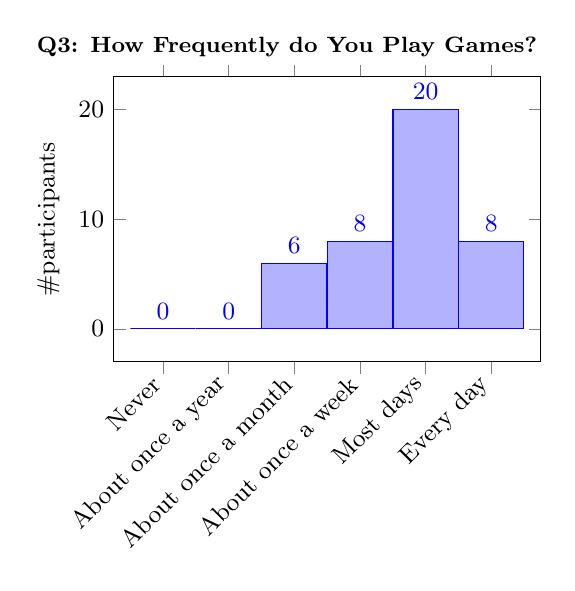
\begin{tikzpicture}
\node[] at (2.2,4) {\textbf{\footnotesize Q3: How Frequently do You Play Games?}};
  \begin{axis}[
    ybar,
bar width=0.83cm,
width = 7cm,
height = 5.2cm,
    enlargelimits=0.15,
    legend style={at={(0.5,-0.2)},
      anchor=north,legend columns=-0.5},
    ylabel={\#participants},
    symbolic x coords={Never,About once a year, About once a month,
		About once a week, Most days, Every day},
    xtick=data,
    nodes near coords, 
	nodes near coords align={vertical},
    x tick label style={rotate=45,anchor=east},
    every axis/.append style={font=\small},
    ]
    \addplot coordinates {(Never,0) (About once a year,0) 
		(About once a month,6) (About once a week,8) (Most days,20) (Every day,8)};
  \end{axis}
\end{tikzpicture}
\hspace*{1cm}
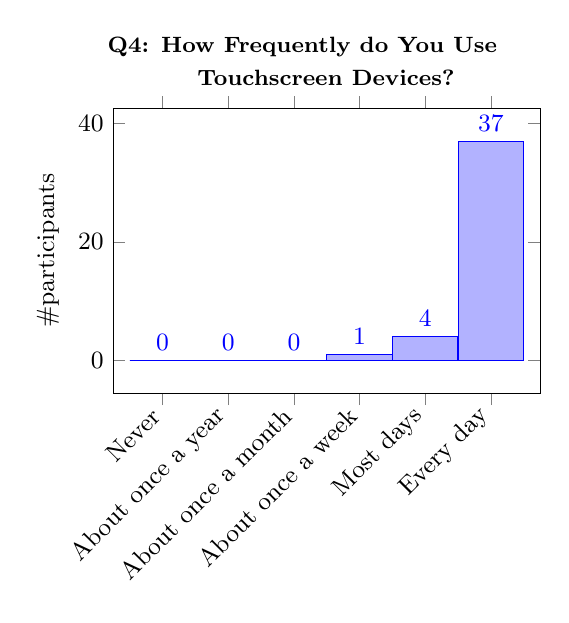
\begin{tikzpicture}
\node[] at (2.4,4.4) {\textbf{\footnotesize Q4: How Frequently do You Use }};
\node[] at (2.7,4) {\textbf{\footnotesize Touchscreen Devices?}};

  \begin{axis}[
    ybar,
    bar width=0.83cm,
    width = 7cm,
    height = 5.2cm,
    enlargelimits=0.15,
    legend style={at={(0.5,-0.2)},
      anchor=north,legend columns=-1},
    ylabel={\#participants},
    symbolic x coords={Never,About once a year, About once a month,
		About once a week, Most days, Every day},
    xtick=data,
    nodes near coords, 
	nodes near coords align={vertical},
    x tick label style={rotate=45,anchor=east},
        every axis/.append style={font=\small},
    ]
    \addplot coordinates {(Never,0) (About once a year,0) 
		(About once a month,0) (About once a week,1) (Most days,4) (Every day,37)};
  \end{axis}
\end{tikzpicture}

\vspace* {0.3cm}
%%%%%%%ROW 2 %%%%%%%%%%
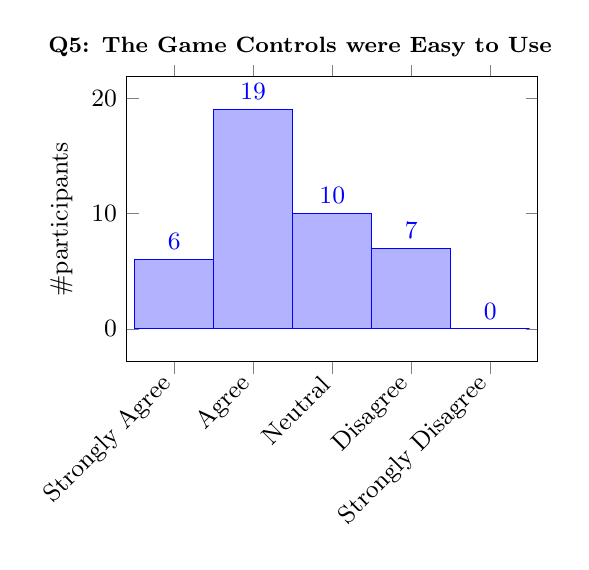
\begin{tikzpicture}
\node[] at (2.2,4) {\textbf{\footnotesize Q5: The Game Controls were Easy to Use}};
  \begin{axis}[
    ybar,
    bar width=1cm,
    width = 6.8cm,
    height = 5.2cm,
    enlargelimits=0.15,
    ylabel={\#participants},
    symbolic x coords={Strongly Agree,Agree,Neutral,
		Disagree, Strongly Disagree},
    xtick=data,
    nodes near coords, 
	nodes near coords align={vertical},
    x tick label style={rotate=45,anchor=east},
        every axis/.append style={font=\small},
    ]
    \addplot coordinates {(Strongly Agree,6) (Agree,19) 
		(Neutral, 10) (Disagree,7) (Strongly Disagree,0)};
  \end{axis}
\end{tikzpicture}
\hspace*{0.8cm}
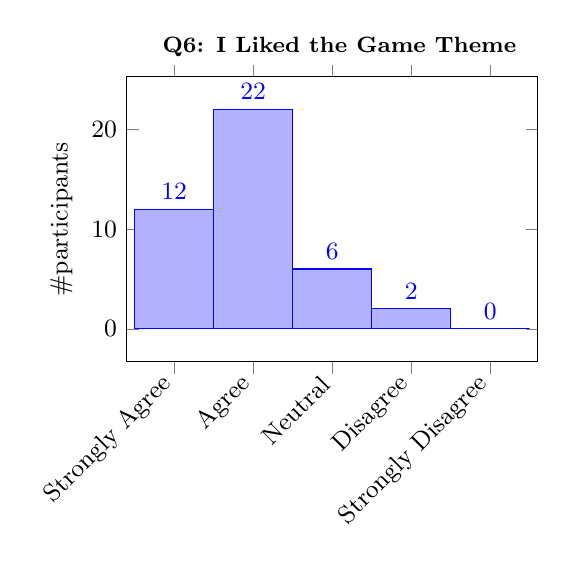
\begin{tikzpicture}
\node[] at (2.7,4) {\textbf{\footnotesize Q6: I Liked the Game Theme }};
  \begin{axis}[
    ybar,
    bar width=1cm,
    width = 6.8cm,
    height = 5.2cm,
    enlargelimits=0.15,
    ylabel={\#participants},
    symbolic x coords={Strongly Agree,Agree,Neutral,
		Disagree, Strongly Disagree},
    xtick=data,
    nodes near coords, 
	nodes near coords align={vertical},
    x tick label style={rotate=45,anchor=east},
        every axis/.append style={font=\small},
    ]
    \addplot coordinates {(Strongly Agree,12) (Agree,22) 
		(Neutral, 6) (Disagree,2) (Strongly Disagree,0)};
  \end{axis}
\end{tikzpicture}
\caption{Frequency of responses for questionnaire questions Q3-Q6}
\label{fig:frequency}
\end{figure}

\begin{description}
\item[Q3) How Frequently do you Play Games?: ]
The response for this question, shown in Figure \ref{fig:frequency}, shows that $86\%$ of those asked play games at least once a week, with the majority playing most days. This result is a positive sign, showing that those in the target age group are likely to relate to a screening test in the form of a game, as they already have a lot of interaction with games.

\item[Q4) How Frequently do you Use Touchscreen Devices?:]
The response for this question, shown in Figure \ref{fig:frequency}, shows that $100\%$ of those asked use touchscreen devices every week, with $88\%$ using them daily. This information confirms that using a touchscreen mobile device was a good choice for the target audience. It also shows that potential users are likely to be familiar with touchscreen concepts, such as the gestures used within the game.

\item[Q5: The Game Controls were Easy to Use]
Figure \ref{fig:frequency} shows that $60\%$ of those asked agreed or strongly agreed that the controls were easy to use. Though this is the majority, it is not as many as hoped and it is important that the users find the controls easy to use to prevent them from becoming frustrated with the game and losing interest. When asked, the majority of participants who chose neutral or disagree said that they found jumping difficult, it may be worth examining other options for the jump control in later versions of the game.

\item[Q6: I Liked the Game Theme]
The responses for this question, shown in Figure \ref{fig:frequency} show that $81\%$ of participants agree or strongly agree with this statement, such a high percentage means the game theme is likely to be suitable for the target audience.

\item[Q7: The Game was too Challenging]
Figure \ref{fig:frequency2} shows that $98\%$ of participants did not agree with this statement and though this is a positive sign, this does not show that the game is the correct difficulty for the target age group, the game must also not be too easy, in order to keep users engaged.

\item[Q8: I Enjoyed Playing the Game]
Figure \ref{fig:frequency2} shows that $83\%$ of participants  agreed or strongly agreed with this statement, a very positive response. In addition, only a single participant felt the experience was negative. 

\item[Q9: The Game Took too Long to Play]
Figure \ref{fig:frequency2} shows that $95\%$ of participants did not agree with this statement, a very good response. For this question, it is important that users do not think the game is too long as they need to be engaged in order to get the most accurate results. It is not of concern that many participants felt the game was too short, as the primary goal of the game is to screen for dyslexia as efficiently as possible.

\item[Q10: The Game was too Easy]
Figure \ref{fig:frequency2} shows that $93\%$ of participants did not feel strongly either way about this statement. The ideal response would be for all participants to feel neutrally about this statement meaning that the game is the correct difficulty. The results for this statement, coupled with the response for Q7, are promising and suggest that the difficultly of the game is inline with what the target audience expect.
\end{description}

\begin{figure}[h]
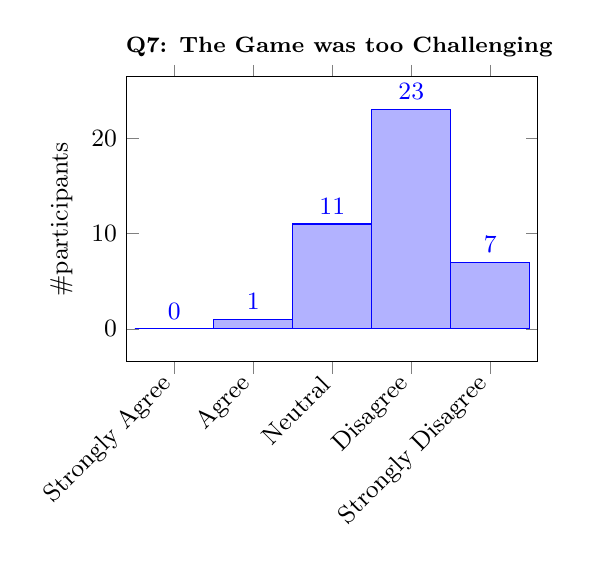
\begin{tikzpicture}
\node[] at (2.7,4) {\textbf{\footnotesize Q7: The Game was too Challenging}};
  \begin{axis}[
    ybar,
    bar width=1cm,
    width = 6.8cm,
    height = 5.2cm,
    enlargelimits=0.15,
    legend style={at={(0.5,-0.2)},
      anchor=north,legend columns=-1},
    ylabel={\#participants},
    symbolic x coords={Strongly Agree,Agree,Neutral,
		Disagree, Strongly Disagree},
    xtick=data,
    nodes near coords, 
	nodes near coords align={vertical},
    x tick label style={rotate=45,anchor=east},
        every axis/.append style={font=\small},
    ]
    \addplot coordinates {(Strongly Agree,0) (Agree,1) 
		(Neutral, 11) (Disagree,23) (Strongly Disagree,7)};
  \end{axis}
\end{tikzpicture}
\hspace*{1cm}
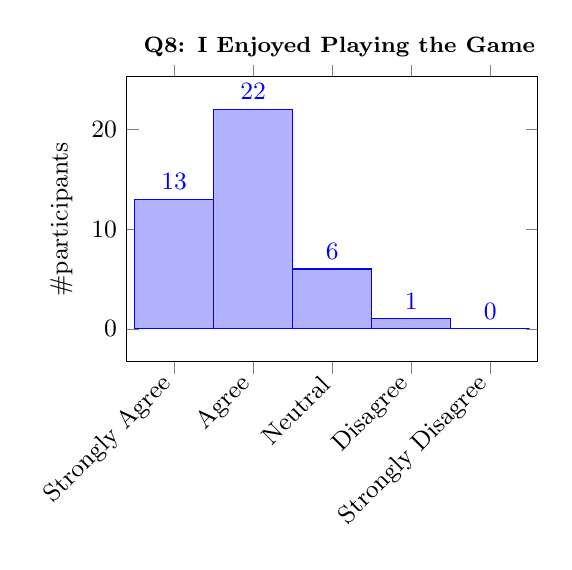
\begin{tikzpicture}
\node[] at (2.7,4) {\textbf{\footnotesize Q8: I Enjoyed Playing the Game }};
  \begin{axis}[
    ybar,
    bar width=1cm,
    width = 6.8cm,
    height = 5.2cm,
    enlargelimits=0.15,
    legend style={at={(0.5,-0.2)},
      anchor=north,legend columns=-1},
    ylabel={\#participants},
    symbolic x coords={Strongly Agree,Agree,Neutral,
		Disagree, Strongly Disagree},
    xtick=data,
    nodes near coords, 
	nodes near coords align={vertical},
    x tick label style={rotate=45,anchor=east},
        every axis/.append style={font=\small},
    ]
    \addplot coordinates {(Strongly Agree,13) (Agree,22) 
		(Neutral, 6) (Disagree,1) (Strongly Disagree,0)};
  \end{axis}
\end{tikzpicture}
\vspace*{0.5cm}
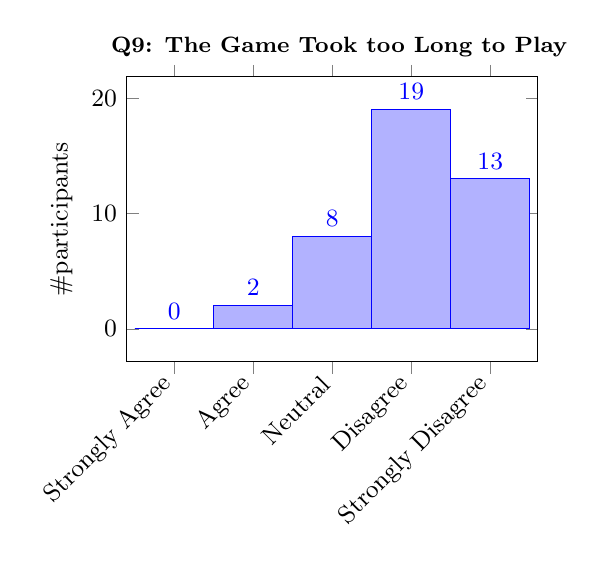
\begin{tikzpicture}
\node[] at (2.7,4) {\textbf{\footnotesize Q9: The Game Took too Long to Play}};
  \begin{axis}[
    ybar,
    bar width=1cm,
    width = 6.8cm,
    height = 5.2cm,
    enlargelimits=0.15,
    legend style={at={(0.5,-0.2)},
      anchor=north,legend columns=-1},
    ylabel={\#participants},
    symbolic x coords={Strongly Agree,Agree,Neutral,
		Disagree, Strongly Disagree},
    xtick=data,
    nodes near coords, 
	nodes near coords align={vertical},
    x tick label style={rotate=45,anchor=east},
        every axis/.append style={font=\small},
    ]
    \addplot coordinates {(Strongly Agree,0) (Agree,2) 
		(Neutral, 8) (Disagree,19) (Strongly Disagree,13)};
  \end{axis}
\end{tikzpicture}
\hspace*{1cm}
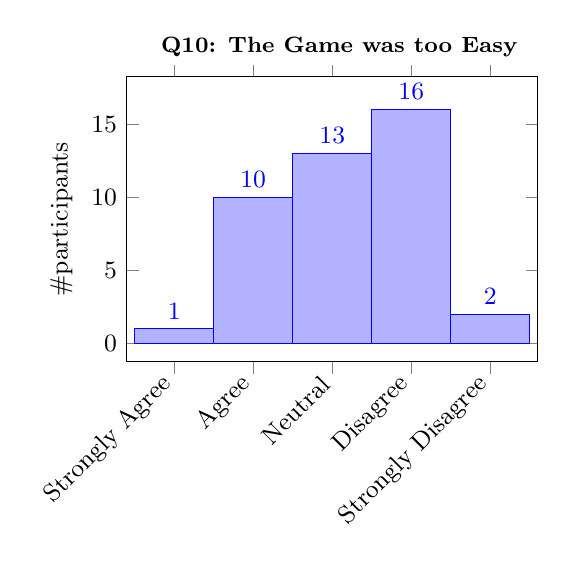
\begin{tikzpicture}
\node[] at (2.7,4) {\textbf{\footnotesize Q10: The Game was too Easy}};
  \begin{axis}[
    ybar,
    bar width=1cm,
    width = 6.8cm,
    height = 5.2cm,
    enlargelimits=0.15,
    legend style={at={(0.5,-0.2)},
      anchor=north,legend columns=-1},
    ylabel={\#participants},
    symbolic x coords={Strongly Agree,Agree,Neutral,
		Disagree, Strongly Disagree},
    xtick=data,
    nodes near coords, 
	nodes near coords align={vertical},
    x tick label style={rotate=45,anchor=east},
        every axis/.append style={font=\small},
    ]
    \addplot coordinates {(Strongly Agree,1) (Agree,10) 
		(Neutral, 13) (Disagree,16) (Strongly Disagree,2)};
  \end{axis}
\end{tikzpicture}
\vspace*{-1cm}
\caption{Frequency of responses for questionnaire questions Q7-Q10}
\label{fig:frequency2}
\end{figure}

\subsection{Identifying Participants with Dyslexia Results}
\label{sec:dyslexiaResults}
In this section the results of the game study are presented and analysed, in relation to null hypothesis \textbf{NH.1}, testing whether significant differences between the performance metrics achieved by the two groups exist, and whether it is possible to correctly classify participants into the correct groups. A summary of the results obtained from the study, are presented in Table \ref{tab:studyRaw} and include basic participant information and game play metrics. 

\tableformat{p{4.5cm}| c c c c c}{
\hline
\rowcolor{gray!30}  & \multicolumn{2}{ c }{With Dyslexia} & \multicolumn{2}{ c }{Controls} & Mann-Whitney U \\ 
\rowcolor{gray!30} Game Metric & Mean & SD & Mean & SD & Significance\\ \hline

 %%Game 1
Time Task 1 & 58.77 & 23.79 & 69.85 & 60.95 & 0.843\\
Errors Task 1 & 1.57 & 1.90  &  2.11 &4.33 & 0.869 \\

 %%Game 2
Time Task 2 (Round 1)  & 59.30 & 33.79 & 53.06 & 27.30 & 0.644\\
Time Task 2 (Round 2)  & 43.01 &  9.78 & 43.04 &  25.59 & 0.574\\

 %%Game 3
Time Task 3  & 44.55  &  15.64 & 38.93 & 12.51 & 0.353 \\
Errors Task 3  & 3.00 & 2.58 & 2.69 &  2.93 & 0.668 \\

  %%Game 4
Time Task 4 & 42.29 & 11.32 & 38.50  & 11.24 & 0.370 \\
Errors Task 4 & 4.86 & 2.91 & 0.86 & 1.06 & \textbf{$<$0.001}\\
Switch Presses Task 4 &  6.71 & 2.43 & 8.54 & 4.88 & 0.426 \\

 %%Game 5
Time Task 5 &  33.54 & 8.87 & 26.73 & 9.48 & \textbf{0.045} \\
Errors Task 5 & 1.00 & 0.82 &  0.83 & 1.20 & 0.370\\
}{Summary of the results obtained by the study, all times are given in seconds. }
{tab:studyRaw}

A \emph{Mann-Whitney U} significance test was performed on each of the game metrics to determine if the observed differences between the results achieved by the two groups are significant. The significance level used was $p=0.05$, such that there is at most a $5\%$ probability that the results are drawn from the same distribution. The results of this significance testing, also shown in Table \ref{tab:studyRaw}, show that two of the eleven performance metrics show significant differences between the two groups: the number of errors made in task 4 and the time taken to complete task 5.

The group with dyslexia made significantly more errors on task 4, the task designed to test visual sequential memory, previous work presented in Chapter \ref{chap:litreview} support this result, suggesting that controls would perform better in this task.
The group with dyslexia were also significantly slower when completing task 5, the task designed to test visual memory. This was also expected, as the research in Chapter \ref{chap:litreview} suggested that the problem of rotating and reversing letters seen in some individuals with dyslexia, could cause them to perform worse than controls in this task.

Having determined which individual tasks identify significant differences between the two groups, the problem can be approached as one of classification:
\cquestion{Can a model be built from the game performance metrics which can predict which class an individual belongs to}

When attempting to answer this question, methods such as \emph{Principal Component Analysis} (PCA) and \emph{Linear Discriminant analysis}(LDA) were considered for data preprocessing. 
PCA reduces dimensionality by identifying a smaller set of variables, which are linear combinations of the original inputs,  which preserve the majority of the variance in the data\cite{PCA}.   
LDA is similar, however, exploits knowledge of the desired output class for each data record by attempting to model the differences between the classes.  
However, both PCA and LDA make a lot of assumptions about the data and are unlikely to be suitable for use on such a small dataset. 

Instead, \emph{Logistic Regression} (LR) was used to create a model capable of classifying the data collected in this study, and to reduce overfitting. 
LR classifies data records by calculating the conditional probability  $P(Y=1|X=x)$, where $Y=1$ is a positive output and in this case means that the participant belongs in the group with dyslexia. $x$ is the dependant variables used as input\cite{LR}, in this case the performance metrics collected during game play. LR allows non-linear relationships between the inputs and the output to be modelled, reducing the inputs to a single probability score, such that individuals what a probability score $\geq0.5$ will be classified in the group with dyslexia. 


Using all of the game metrics as inputs to the LR model is likely to seriously overfit to the data, and impede generalisation. Instead, only the variables which identified significant differences between the two groups were used for the model, the number of errors made in task $4$ and the time taken to complete task 5.

An LR model was fitted to the data using the \emph{Binary Logistic Regression Tool} available in the \emph{SPSS Statistics} software. Step 0 of the model, with no inputs included as predictors, achieved $83.3\%$ accuracy by assuming that all participants fell into the control group. One further step was performed, adding the number of errors made in task $4$ to the model as a predictor, no further steps were performed as adding the time taken to complete task $5$ made no significant difference to the model.

The final model equation, shown in equation \ref{eq:model}, can be used as part of equation \ref{eq:predict} to find the probability that an individual with performance metrics $x$ belongs in the group with dyslexia. When classifying, a probability $<0.5$ means the individual belongs in the control group, a probability $\geq 0.5$ means that the individual belongs in the group with dyslexia.
When examining the data collected in this study, this model achieved an accuracy of $95.2\%$ when attempting to classify participants into one of the two classes. $5$ of the $7$ participants with dyslexia were correctly classified, all other participants were classified as controls.

\begin{equation}
\small
\mathrm{logit}(p(x))= -6.921  + 2.140 \cdot E_{4} \label{eq:model}
\end{equation}
 \begin{center}
	\vspace*{-0.1cm}
	\small
   where $E_{4}$ is the number of errors made in task 4.
   \end{center}
   
   \begin{equation}
\small
p = \frac{\mathrm{e}^{\mathrm{logit}(p(x))}}{1 + \mathrm{e}^{\mathrm{logit}(p(x))}}
\label{eq:predict}
\end{equation}
   
\subsection{Discussion}
\label{sec:disscussion}
In this section the results presented in section \ref{sec:results} are discussed in order to establish their meaning.
 
\subsection{Discussion of the Significance and Logistic Regression Results}

Section \ref{sec:dyslexiaResults}, found that using the \emph{Mann-Whitney U} significance test, significant results were seen for two of the game play metrics, meaning there is at least a $95\%$ confidence that the values achieved by the two groups are drawn from different distributions.
The \emph{Mann-Whitney U} test was chosen as it is a non-parametric test capable of comparing two independent classes, there was no reason to believe that the data collected in this study had a normal distribution therefore tests such as the \emph{Students T-Test} would have been unsuitable. 
These results mean that null hypothesis \textbf{NH.1} could be rejected, as there is an observable and indeed significant difference between the results achieved by the two groups, although only in two of the eleven metrics. 
Though this is a positive sign, it is important to consider that the dataset used for this analysis is very small and that only $7$ of the $42$ participants belonged in the group with dyslexia. This means that it is unlikely that the sample used in this study is truly representative of the actual population, that said, the results provide a good basis for further work and it would be interesting to see if this effect is still observed with a much larger dataset.


The results of the \emph{Logistic Regression} analysis showed that a model can be created using equations \ref{eq:model} and \ref{eq:predict} which can achieve $95.2\%$ accuracy, utilising a game play performance metric as a predictor. This again means that null hypothesis \textbf{NH.1} could be rejected, as the model uses a function of the game performance metrics to classify participants.
This does not ensure that the model will generalise with a high accuracy to new data as it is likely that, due the small size of the dataset, the model has overfitted to the provided data points. To test the model, unseen data should be presented to it and it should be judged on how well it classifies this data. Ideally this would have been done as part of this project, however, the size of the group with dyslexia is already very small and there was not enough data to exclude samples from the model for use in testing.

What the model does show is promise. The model achieved a high level of accuracy and the null hypothesis could be rejected, meaning there is reason to believe that the game is capable of separating the two classes and thus being used a screening test. The only way to determine whether the model will generalise is to collect more data and test it.
 
It is worth noting that it was very difficult to find participants with dyslexia within the timeframe of the project and that, despite every effort being made including involving schools in the study, only $7$ participants were found that had been diagnosed with dyslexia, making it difficult to come to any definitive conclusions about the capabilities of the game. 
 
\subsection{Discussion of the Questionnaire Results}
The questionnaire results, presented in section \ref{sec:questionResults}, were generally positive, suggesting that the decision to embark on this research was justified, with nearly all participants using games regularly and enjoying the produced game. Results also suggest that, on the most part, the decisions made concerning the games structure, theme, and content were correct. 
When considering the controls of the game the questionnaire found that some players struggled with the jump control. Though this may not seem important as it is not part of a dyslexia screening task, users struggling to navigate the platform game could result in them having an overall negative experience with the game and perhaps not even finishing it. It is therefore important that the difficulties with the jump control are addressed. To ensure issues with the game controls did not bias the results, effecting one group significantly, the answers to this question were tested for significance. No significant difference between the answers given by those with dyslexia and controls was identified, with a significance score of $0.620$. 

The majority of participants thought that the game did not take too long to play, suggesting that it might even be too short. This is not a concern at this time as the priority at this stage is to refine the predictive power of the game. However, the game ending prematurely may leave some users feeling dissatisfied with the experience and have a negative effect on public opinion. It may therefore be worth examining the duration of the game, or perhaps creating a more interesting and fulfilling ending, in later versions.

The number of questions in the questionnaire was limited, so as not to overwhelm younger participants. It may have been beneficial to have asked for more information, in particular to gain insight into the users opinions of the screening tests. This would help to determine if the screening tasks which show significant differences between the groups are well received by users.
 
\section{Conclusions}

In summary, this project aimed to create ``A Serious Game For Aiding the Screening of Dyslexia in Children and Young Adults'' in the hope of replacing the current screening tests. The work completed has gone a long way towards achieving this goal, despite the time and resource limitations. 

In depth analysis was performed in Chapter \ref{chap:litreview}, reviewing the breadth of current knowledge surrounding both dyslexia and games. This knowledge was then utilised to create a game design, specifically engineered to include tasks designed to identify differences between those with and without dyslexia. 
This design was then rapidly realised, through careful planning and adhering to software engineering principles and methodologies, including the use of TDD, extracting requirements from use cases, and examining the important quality attributes associated with the system.
 
The game implementation was then tested, both for usability and validity. The results of this testing were positive, however, due to lack of data cannot be taken to be definitive. Some of the screening tasks, have shown that they may be capable of distinguishing between the the two groups, and have allowed null hypothesis \textbf{NH.1} to be rejected. Usability testing revealed the strengths and weaknesses of the game design and implementation, with users enjoying the game and the theme as a whole, but finding the controls difficult to grasp.

Overall, though no definitive conclusions could be reached about the games effectiveness as a screening test, due to lack of data, the game certainly proved itself to be an enjoyable experience for users and identified the tasks most likely to have predictive power. Hopefully, with further research, the game developed in this project could be a contender to the current dyslexia screening tests, making the experience more enjoyable and accessible for all.

\subsection{Further Work}
The work completed in this project could be extended in a number of ways, these can be split into three groups: the game platform, the screening tasks, and the data.

\subsubsection{Game Platform and Hardware}
Currently the game is only designed to run on the Apple iPad and iPad Mini. In order for the game to be as accessible as hoped for, it would need to be ported to other platforms and hardware. Possible targets include the Apple iPhone and Android devices. Porting the game to the iPhone would be reasonably straight forward as the majority of the existing implementation could be reused, although issues may be faced when considering the difference in screen size.
Porting the game to Android would be a more difficult task and it is recommended that the game support only the latest versions of the operating system, as it would be difficult to handle the fragmentation if lower versions were included.

\subsubsection{Screening Tasks}
There were a number of screening task ideas included in Chapter \ref{chap:design} which were not included in the game implementation. It may be the case that some of these tasks, or perhaps completely new tasks, would be better at finding differences between the two groups than some of the tasks that have been included. This is worth exploring as model accuracy is important, therefore, anything that could increase this is also important.

In addition, it may also be beneficial to increase the difficulty of the tasks which did not find significant differences between the groups. It may be that they are capable of finding differences but have not been implemented at the correct difficulty level to make those differences apparent. Since participants did not find the game too challenging, it should be possible to do this without negatively impacting the users experience.

\subsubsection{Data}
There are two ways in which the work conducted in this project could be advanced by collecting additional data. 
The first is to better test the model, or improve it. Currently the model relies on very little data and is likely to be overfitted. More data is required in order to properly test it and produce definitive results.

Data could also be collected on an ordinal scale, ranking participants given that the severity of their dyslexia is known. This data would be useful as currently even if the model was capable of generalising, it only produces a binary output. Knowing more information about an each individuals place of the dyslexic continuum could help teachers prioritise and help those most in need first.

\bibliography{references}
\bibliographystyle{IEEEtran}
\section{Appendix}
\end{document}


